\chapter{State of the Art}


The research and interest in humanoid robotics has greatly increased over the last few years, but inspite of the current
abundance of the humanoid robots, their utility is still very limited. One of the most important trials, \textit{DARPA 
Robotics Challenge (DRC)} in 2013 listed a pack of capabilities and robustness that humanoid robots lacked when performing 
different tasks. Each task of this challenge should last only up to 30 minutes. These tasks will take less than a minute 
for a human to complete which  explains the powerlessness of the robots. This chapter briefly explains different control 
strategies that has been carried to keep balance and to handle robot dynamics in humanoid robots.

\section{Approaches in Humanoid Robot Control}

Different methods has been used to make a robot move depending on the application, the complexity of the task, and even
the specific nature of the robot. The main control methods used for the humanoid robots are as follows: Motion planning,
Kinematic Approach, Dynamic Approach and Optimal Control. Each of the methods and its recent development are discussed
below.

\subsection{Motion Planning}

Motion Planning as the name suggests a method where a robot automatically finds its desired or goal state from its initial
configuration. For instance, consider a hand moving from it's current pose to another pose, motion planning allows to move to
goal pose considering the presence of obstacles and consumption of time and energy. Currently, there are many applications in 
industrial robots and mobile robots where the robot motion is planned within both structured and non-structured environment. 

 

Even though, motion planning and its researches are progressing majorly within past decades, the recent approaches are combined
with artificial intelligence, advantages of computer technology and mathematics. The main approaches can be found in books such as 
\cite{Latombe,LaValle2006PlanningA}. An desirable concept in motion planning is \textit{Configuration Space (CS)}, which is the set
of all possible configurations for a robot to attain. For a robot with \textit{n} independent degrees of freedom, \textit{CS} is an 
\textit{n}-dimensional manifold $\mathbb{M}$ that contains all the desired configurations $q \in \mathbb{M}$ of the robot. The importance
of \textit{CS} is that changes the problem of moving a body in \textit{SE(3)} to moving a point in \textit{CS}. The summary of this
section is sourced from the literature work \cite{ramosponce}. Then there exists,

\begin{itemize}
    \item $\mathit{CS_{obs}}$ is the \textit{Obstacle Configuration Space} formed to generate self-collision or obstacle collision free set of
     configurations such that $\mathit{CS_{obs}} \in \mathit{CS}$.
     \item $\mathit{CS_{free}}$ is the \textit{Free Configuration Space} which holds the set of configurations for a freely roaming robot such that 
     $(\mathit{CS_{free}} \bigcup \mathit{CS_{obs}}) \cap \mathit{CS} $.
\end{itemize}

Using these configurations, the problem of motion planning can be stated as finding the continuous path $p(t)$ through the desirable configurations from initial
state $q(0)$ to goal state $q(f)$ avoiding collisions, that is $p: [0, 1]  \rightarrow \mathit{CS_{free}}$ where $t$ defines time parameterization.


\subsubsection{Generic methods}

The solution to motion planning problem can be processed through classical approaches using deterministic, sampling-based or path optimization algorithms. 
Each of the types are briefed below.

\begin{figure}[h!]
    \centering
    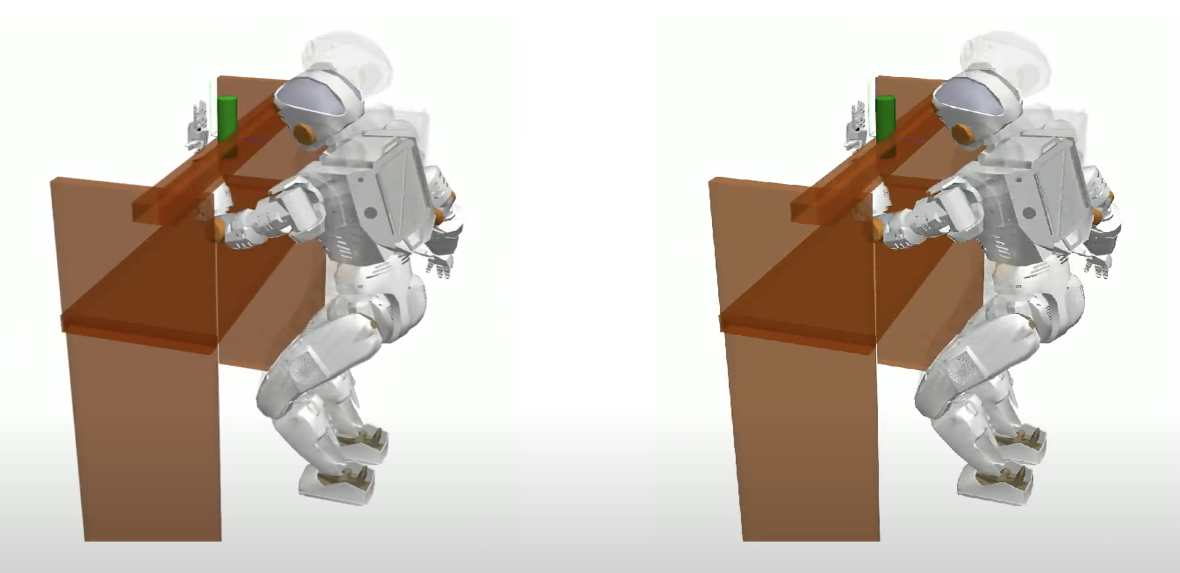
\includegraphics[scale=0.3]{images/motion-planning.png}\hfill
    \caption{Sampling based motion planning of NASA Valkyrie \cite{Vijayakumar}}\hfill
    \label{motion-planning}
\end{figure}

\begin{enumerate}
    \item \textit{Deterministic algorithms -} The deterministic algorithms are developed such that it computes the valid path everytime knowing almost
    all the variables of the environment. Methods such as \textit{cellular decomposition, Voronoi diagrams, visibility graphs, potential fields and Canny's algorithms}
    rely on
    mathematical construction of the environment with the obstacles and provide $\mathit{CS_{obs}}$. Although these algorithms are complete, the computation
    of high-dimensional space is expensive and the environments are always not deterministic.

    \item \textit{Sampling based algorithms -} These algorithms mostly approximate the connectivity of $\mathit{CS_{free}}$ through random sampling configurations
    from $\mathit{CS}$ and rejecting the configurations using boolean collision detection techniques. The main examples are  \textit{Probabilistic Maps and
    Rapidly-exploring Random Trees(RRT)} in combination with Voronoi diagrams promotes the obstacle avoidance configurations for a robot. The main advantage of
    sampling based algorithms are to handle the higher dimensional configuration space recovering a higher degree of completeness.

    \item \textit{Path optimization algorithms -} These algorithms provide optimization in terms of path planning and trajectory planning starting from a valid
    initial state to its goal position with the desired configurations. \textit{Greedy optimization} tries to directly connect the start configuration to 
    its goal state that generates a collision free shortest path by discretizing the path into \textit{n} closest goal configuration relative to previous 
    configuration.
\end{enumerate}

\subsubsection{Motion Planning in Humanoid robots}

Classical motion planning techniques determine collision free trajectories considering only the geometric model of the robot. However the control of
polyarticulated system needs the synthesis of robot models that describe the effect of joint variations on the whole robot configuration. In both the case,
for instance considering an arm moving to it's goal position, the robot tends to make it more unusual, inefficient and unnatural movements. To overcome these 
problems, geometric models are replaced with kinematic models, dynamic models or optimal control and trajectories are generated. Additional constraints like
multiple contacts and dynamic balance of the system are considered. For instance, motion primitives that have been predefined by a human expert based on prior
knowledge can be used to guide the planner \cite{zhang2014motion}. 

 

In case of humanoid walking, the planner can be generated using deterministic approaches with dynamic alterations of the foot transition model considering
the smooth transition of the trajectories for posture transitions. For these cases, sampling-based algorithms are considered to improve the degree of completeness.
Either way, the higher dimensional configuration space is handled so that the problem is solved successively. An example is presented in \cite{yoshida2008planning} where a 36 degree of freedom
robot is reduced to a 3 degrees of freedom bounding box and a PRM is applied for the path planning problem of the box. Another example is to present the
constraints in the form of sub-manifolds of \textit{CS} where a union of separate manifolds like contact limb position and static balance constraints can be 
used to plan the configuration space. In such cases, static balance control in humanoid robots and other legged robots can be obtained \cite{hauser2010multi}.

\subsection{Kinematics Approach}

Generally, \textit{kinematics} is defined as a branch of science which deals with the study of the position, velocity and acceleration of a mechanical system without
considering forces and the dynamic properties of the system (such as mass or inertia) that generate the motion. In humanoid and manipulator robots, the system is 
represented as rigid bodies composed of actuators and sensors. In contrast with the manipulators, the humanoid robots are not fixed to any environment and are highly mobile.
This makes the humanoids (or humanoid robots) more redundant than the manipulators. This section briefs the state of the art and concepts of kinematic approach used in
humanoid control.

\subsubsection{Basic Concepts}

The \textit{joint space} is also called as \textit{configuration space}, of a robot with $n$ degrees of freedom (DoF) is a \textit{n}-dimensional manifold $\mathit{Q}$ containing 
all the possible joint values for a joint $q$ can take. For humanoid robots, this space can be generalized to the operational points \cite{khatib1987unified}, which can represent any part of the body
that may be of interest. In robotics, there exists four subdomains of kinematics namely,  \textit{\textit{(i)} forward kinematics (or direct geometry), \textit{(ii)} inverse kinematics
(or inverse geometry), \textit{(iii)} forward differential kinematics (or simply forward kinematics), and \textit{(iv)} inverse differential kinematics (or simply inverse kinematics).}

\begin{itemize}
    \item \textbf{Direct Geometric Model:} For a robot with $n$ DoF in a $n$-dimensional joint space such that $q \in Q$, there exist a pose $x \in \mathit{SE(3)}$ represented as
    $$x = f(q)$$ described by a map $f:Q \rightarrow \mathit{SE(3)}$.
    
    \item \textbf{Inverse Geometric Model:} For a robot with $n$ DoF in a $n$-dimensional joint space with $q \in Q, x \in \mathit{SE(3)}$, the joint space can be represented from 
    a given pose for a certain operational point as $$q = f^{-1}(x)$$ described by a map $f: \mathit{SE(3) \rightarrow Q}$. But there is a possibility for non-unique solution or 
    non-existing solution (known as singularity).

    \item \textbf{Forward Kinematic Model:} For a robot with $n$ DoF in a $n$-dimensional joint space such that $q \in Q, x \in \mathit{SE(3)}$, the operational twist $\xi \in
     \mathit{SE(3)}$ due to the joint variation $\dot{q}$ is described as $$\xi = J(q)\dot{q}$$ Here, $J$ is the basic Jacobian such that $J : T_q(Q)$ where $T_q(Q)$ is the tangent 
     space of the $Q$ space. Instead, the Jacobian $J$ can be formulated analytically using the pose variation $\dot{x}$ and joint variation $\dot{q}$ as $$\dot{x} = \frac{\partial x}{\partial 
     q}\dot{q} \quad \mathnormal{or} \quad \dot{x} = J\dot{q}$$ then $J$ is the task Jacobian.

     \item \textbf{Inverse Kinematic Model:} For a robot with $n$ DoF in a $n$-dimensional joint space such that $q \in Q, x \in \mathit{SE(3)}$, finding the joint variations $\dot{q}$
     that produce a pose variation $\dot{x}$ of the end effector as $$\dot{q} = J^{-1} \dot{x}$$ and it can be solved iteratively.
\end{itemize}

\subsubsection{Kinematic Control of Redundant robots}

In general, the kinematic control involves a reference planner or trajectories $q_{ref}(t)$ in $\mathit{SE(3)}$ for which the robot joint trajectory $q(t)$ is evaluated against attaining
the objective. Consider a task $i$ in a robot with $n$ DoF, then the Jacobian is of size $m \times n$ and the robot is redundant when $(n > m)$ \cite{nakamura1990advanced}. The joint variations $\dot{q}$ can be represented
if

\begin{itemize}
    \item $(n > m)$. For task $i$, there exists a degree of redundancy $n-m$ for which the joint variation based on lease square method can be given by $$\dot{q} = J_i^+\dot{x_i} + (I_n - J_i^+J_i)z_i$$
    where $J_i^+ = J_i^T(J_iJ_i^T)^{-1}$ is the pseudo inverse of $J_i$, $I_n$ is the identity matrix of size $n$ and $z_i$ is an $n$-dimensional arbitrary vector. The first term in the above equation
    is to minimize the norm solution while the second term is to find all possible solutions. 

    \item $(n = m)$. The degree of redundancy is $0$ and the joint variation can be defined as $$\dot{q} = J^{-1} \dot{x}$$ Note that the Jacobian here is a non-singular matrix.
    \item $(n < m)$. There doesn't exist any redundancy and no solution is found in this case.
\end{itemize}

For multiple tasks, the probability of finding a suitable solution decreases as the preceding tasks influence the current task, in other words, consider two tasks 1 and 2 for a redundant robot. There 
exist a solution for two tasks $x_1 = f_1(q)$ and $x_2 = f_2(q)$ with task priority for $x_1$ and $x_2$ respectively. First the variation $q$ that solves the task according to the priority is 
determined from the differential equations by,

\begin{equation}
    \delta x_1 = J_1\delta q 
    \label{task1}
\end{equation}
\begin{equation}
    \delta x_2 = J_2\delta q 
    \label{task2}
\end{equation}

Then the joint variation $\delta q$ for task $1$ has infinitely many solutions and is given by

\begin{equation}
        \dot{q} = J_i^+\dot{x_i} + (I_n - J_i^+J_i)z_i 
        \label{jvariation}
\end{equation}

Solving \ref{jvariation} and \ref{task2} for $z_1$ arbitrary vector,

\begin{equation}
    z_1 = \hat{J_2^+}(\delta x_2 - J_2J_1^+ \delta x_1) + (I_n - \hat{J_2^+}\hat{J_2})z_2
\end{equation}

where $\hat{J_2} = J_2(I_n + J_1^+J_1)$ and $_2$ is an $n$-dimensional arbitrary vector. Then the solution of joint variation for the two priority tasks can be given by 

\begin{equation}
    \delta q = J^+_1 \delta x_1 + \hat{J_2^+}(\delta x_2 - J_2J_1^+ \delta x_1) + (I_n - J^+_1J_1)(I_n - \hat{J_2^+}\hat{J_2})z_2
\end{equation}

\subsubsection{Generalized form of Task Priority}



\subsubsection{Kinematic Control in humanoid robots}

Humanoid robots as a rigid body representation, from a kinematic point of view present a tree-like structure that includes multiple connected chains, and a high number of DoF. This results in 
higher degree of redundancy with respect to most tasks, in which case the robot is said to be under-constrained. Therefore, methods developed for generic redundant robots are usually applied in humanoid robotics
with some adaptations or additions. Due to the complexity of the kinematic configuration, closed-form solutions for the IK problem are usually very complex, but recently some classical methods 
have been used and modified, to obtain closed equations for specific humanoid robots which are treated as a composition of several kinematic chains. However, methods based on 
instantaneous IK, which compute an increment in q, are usually preferred. This linearization of the problem offers an infinite number of feasible solutions for humanoid robots: there exist different
joint updates that achieve the same task. This leads to the possibility of performing different tasks at the same time, and the IK control must be capable of properly handling them.

 

Methods based on task-prioritization solve these problems and have become the preferred techniques in IK control. They can even be considered as the current “state of the art” in humanoid 
robotics control due to their relatively low computational cost, their straightforward implementation, and the maturity of the approach. Several works with different humanoid platforms use this 
methodology to solve the redundant IK problem at the velocity level using only equality constraints \cite{gienger2005task,yoshida2006task,mansard2007task}. For imposing inequality constraints 
to the control framework at any hierarchical level, a sequence of optimal resolutions for each priority level has been proposed in \cite{kanoun2009prioritizing}, a more efficient computation based on orthogonal 
decompositions can be found in \cite{escande2013planning} and a smooth interchange between priority of consecutive prioritized tasks is introduced in \cite{jarquin2013real}.

\subsection{Dynamics Approach}

Dynamics is the study of the relation between the robot motion and the generalized forces that act on the robot generating that motion. This relation considers parameters such as lengths, 
masses and inertia of the elements composing the robot.



\subsubsection{Basic Concepts}

In the dynamic model, the motion is represented through joint variables acceleration $\ddot{q}$, or operational points acceleration $\ddot{x}$. For rotational joints, the generalized forces are equivalent to 
the joint torques, and for prismatic joints they are the joint forces. There are two main problems in dynamics:

\begin{itemize}
    \item \textbf{Forward Dynamics:} It expresses the motion of the robot as a function of the generalized forces applied to it.
    \item \textbf{Inverse Dynamics:} It expresses the generalized forces acting on a robot as a function of the robot motion.
\end{itemize}

There exist two main formulations to compute the robot dynamic model: the Lagrange approach, and the Newton-Euler approach. The Lagrange approach's main advantage is the clear separation 
of each component of the model; but in general, it is computationally expensive.
The Newton-Euler approach does not provide a clear separation of the terms but due to its recursivity a lower computation time can be obtained. Thus, it is 
the preferred implementation for computer calculations. The most used algorithms for this approach can be found in \cite{featherstone2000robot,featherstone2014rigid}. The Lagrange method and 
Newton Euler's method are detailed in the chapter \ref{chapter-3} under section \ref{dynamic-consideration}.


The introduction of centroidal momentum and centroidal dynamics based on the Centre of Mass (CoM) of a system is particularly a import concept since the humanoids build large momenta(so far only
angular momentum is larger and linear momentum on legger humanoids are not upto the mark). The dynamic model of a robot can be expressed in two ways depending on the spaces that are used to describe the motion and the control input. The two approaches are: the joint space formulation, and the operational space 
(or task space) formulation. The joint space formulation is the classical approach and uses the joint space acceleration to specify the motion, and the generalized forces acting on the actuated joints 
to describe the control. The operational space formulation represents the motion directly using the task space acceleration, which needs a reformulation of the forces as task space generalized 
forces.

\subsubsection{Dynamic Control in Humanoid Robots}

For a humanoid robot, classical dynamic control techniques are not sufficient since coordination of the motion is required, environmental forces need to be considered, and balance has to be kept at all 
time. For the robot balance, a stability criterion such as keeping the CoM or the ZMP inside the support polygon must be enforced. For planar surfaces, the constraint on the 
ZMP implies a control of the contact forces. Thus, the interaction with the environment is always present since the feet are in contact with the ground and additional contacts of other parts of the robot 
body might also be necessary. These contacts generate an effect on the joints generalized forces, which cannot be controlled using only kinematic methods but with dynamic approaches. The dynamic control 
ensures the physical feasibility of the motion and allows for faster movements without losing balance.

The Operational Space Inverse Dynamics (OSID) is a more specific framework for controlling the whole-body of humanoid robots considering contacts and a set of different constraints. This approach
proposed in \cite{khatib2004whole,sentis2005control} is based on a two stage mapping to obtain consistent contact forces and is equivalent to successive projections onto the nullspaces of the previous tasks. Therefore, 
new tasks can be added without dynamically interfering with higher priority tasks. Other methods use the OSID within frameworks that 
involve some type of optimization to find the local solution. The most popular approaches use Quadratic Programming (QP), which allows for the specification of both equality and inequality constraints.
The latter type of constraints is fundamental in humanoid robotics to directly model unilateral contacts, and it is also important to properly specify some particular tasks. Although the previous approaches exploit the full robot dynamics, 
the angular momentum is not explicitly controlled within these frameworks. Nevertheless, it has been shown that the angular momentum 
is a natural and important part of human motion, specially when performing complex and fast movements \cite{popovic2004angular}. 

\subsection{Optimal Control}

Optimal control, also known in robotics as trajectory optimization or trajectory filtering, consists in finding a trajectory and its associated control law (policy) that satisfies some predefined 
optimality criterion. In general mathematical terms, it concerns the properties of control functions which, when inserted into a differential equation, give solutions that minimize a cost or measure
 of performance. But it also concerns optimization problems with dynamic constraints which might be functional differential equations, difference equations, partial differential equations or equations 
 with another form. This section is summarized from the literature work \cite{ramosponce} which provides a brief overview of optimal control in humanoid robots.


\subsubsection{Optimal Control in Humanoid Robots}

In robotics, optimal control can be used to find the trajectories from an initial posture to a final desired posture, specified as a whole or as a set of sub-objectives, satisfying certain constraints.
Very fast and powerful movements can be generated with optimal control, which can comprehend the problems of inverse kinematics or inverse dynamics and can therefore pro- duce better movements. The 
problem with IK and OSID alone is their inability to properly handle the CoM accelerations, thus overrestricting the motion. A solution typically relies on a dedicated submodel, like a linearized 
inverted pendulum \cite{kajita2003biped} to capture the future of the system, but this ad-hoc resolution increases the control architecture complexity. Thus, using these schemes the future states of the system
can be somehow predicted, but dedicated submodels would need to be developed for each case. However, optimal control is the most suitable approach that allows to take into account all the constraints
at the same time. In fact, optimal control can automatically generate the proper trajectory for the CoM in order to achieve fast movements: it acts as a classical pattern generator used for walking
schemes, but additionally incorporating whole-body motion. A serious challenge to optimization-based approaches in robotics is that the timescales of the dynamics are faster than in other applications 
and need a faster response. Currently, the main problem is the computational time, due to the high number of DoF, that forbids its use in real-time applications.

The main drawback of optimal control is the curse of dimensionality, which is particularly important for humanoid robots whose state space is so large that no control scheme can explore all of it in advance and 
prepare suitable responses for every situation. It would be desirable to obtain optimal control in real time; however, currently there is no approach that can achieve this: the solutions are very time consuming 
and generic solvers tend to get stuck into local minima or they even return trivial solutions. The problem of finding the proper formulation and resolution of optimal control is still an open issue in robotics.

\section{Approaches in Humanoid Balance Control}

\subsection{Linear Inverse Pendulum Approach}

Consider a simple inverted pendulum model as in figure [\ref{ipm}] with mass $m$ and link length $l_1$, the kinematics and dynamics for the model can be represented as,

\begin{figure}[h!]
    \centering
    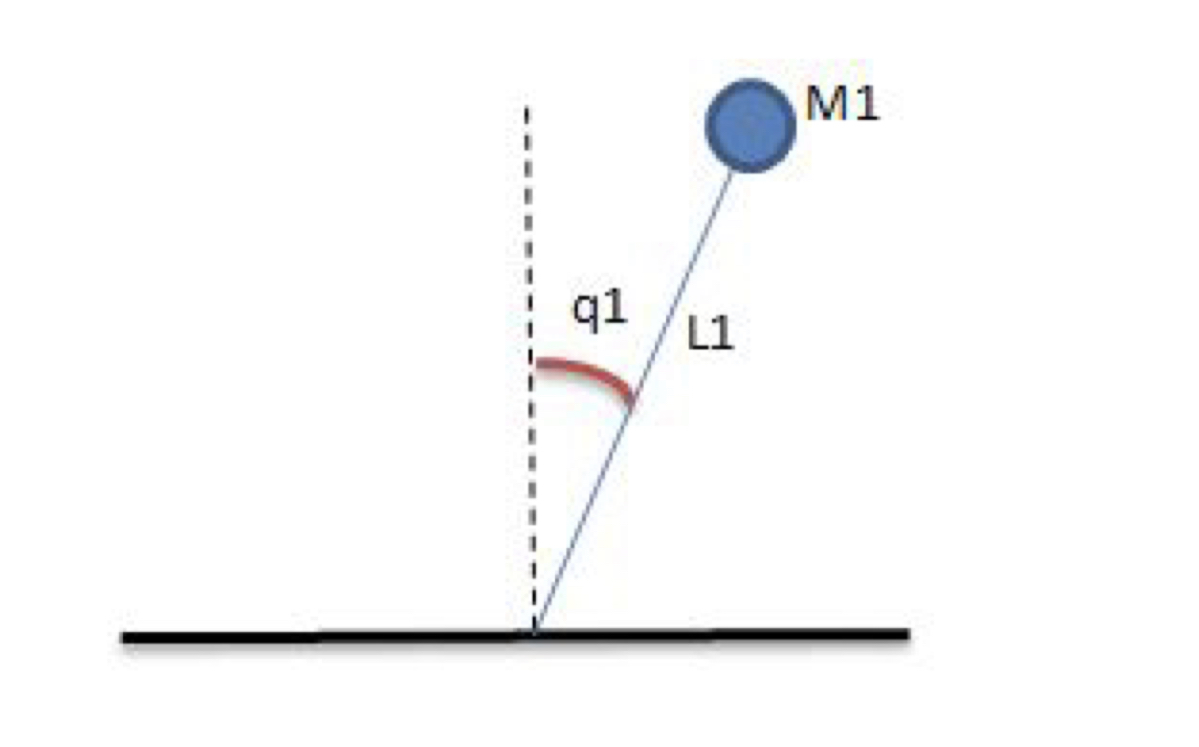
\includegraphics[scale=.15]{images/ipm.jpeg}\hfill
    \caption{Simple Inverse Pendulum Model}\hfill
    \label{ipm}
\end{figure}

Position:
\begin{equation}
\begin{split}
    x_1 &= -l_1\sin{q_1} \\
    y_1 &= l_1\cos{q_1}
\end{split}
\end{equation}

Velocity:
\begin{equation}
\begin{split}
    \Dot{x_1} &= -l_1\cos({q_1})\Dot{q_1} \\
    \Dot{y_1} &= -l_1\sin({q_1})\Dot{q_1}
\end{split}
\end{equation}

Acceleration:
\begin{equation}
\begin{split}
    \Ddot{x_1} &= l_1 \sin{(q_1)}\Dot{q_1}^2 - l_1\cos{(q_1)}\Ddot{q_1} \\
    \Ddot{y_1} &= -l_1 \cos{(q_1)}\Dot{q_1}^2 - l_1 \sin{(q_1)}\Ddot{q_1}
\end{split}
\end{equation}

Forces and Torques:
\begin{equation}
\begin{split}
    m_1\Ddot{x_1} &= F_{x1} \\
    m_1\Ddot{y_1} &= F_{y1} - m_1g
\end{split} 
\end{equation}
\begin{equation}
    \tau_1 = m_1l_1^2\Ddot{q_1} + m_1gl_1\sin{q_1}
\end{equation}

where $F_{x1}$ and $F_{y1}$ represent the reaction forces on the link from the fixed point.

\subsection{Double Inverse Pendulum Approach}

Consider a double inverted pendulum model as in figure [\ref{dipm}] with mass $m$ and link lengths $l_1$ and $l_2$, the kinematics and dynamics for the model can be represented as,

\begin{figure}[h!]
    \centering
    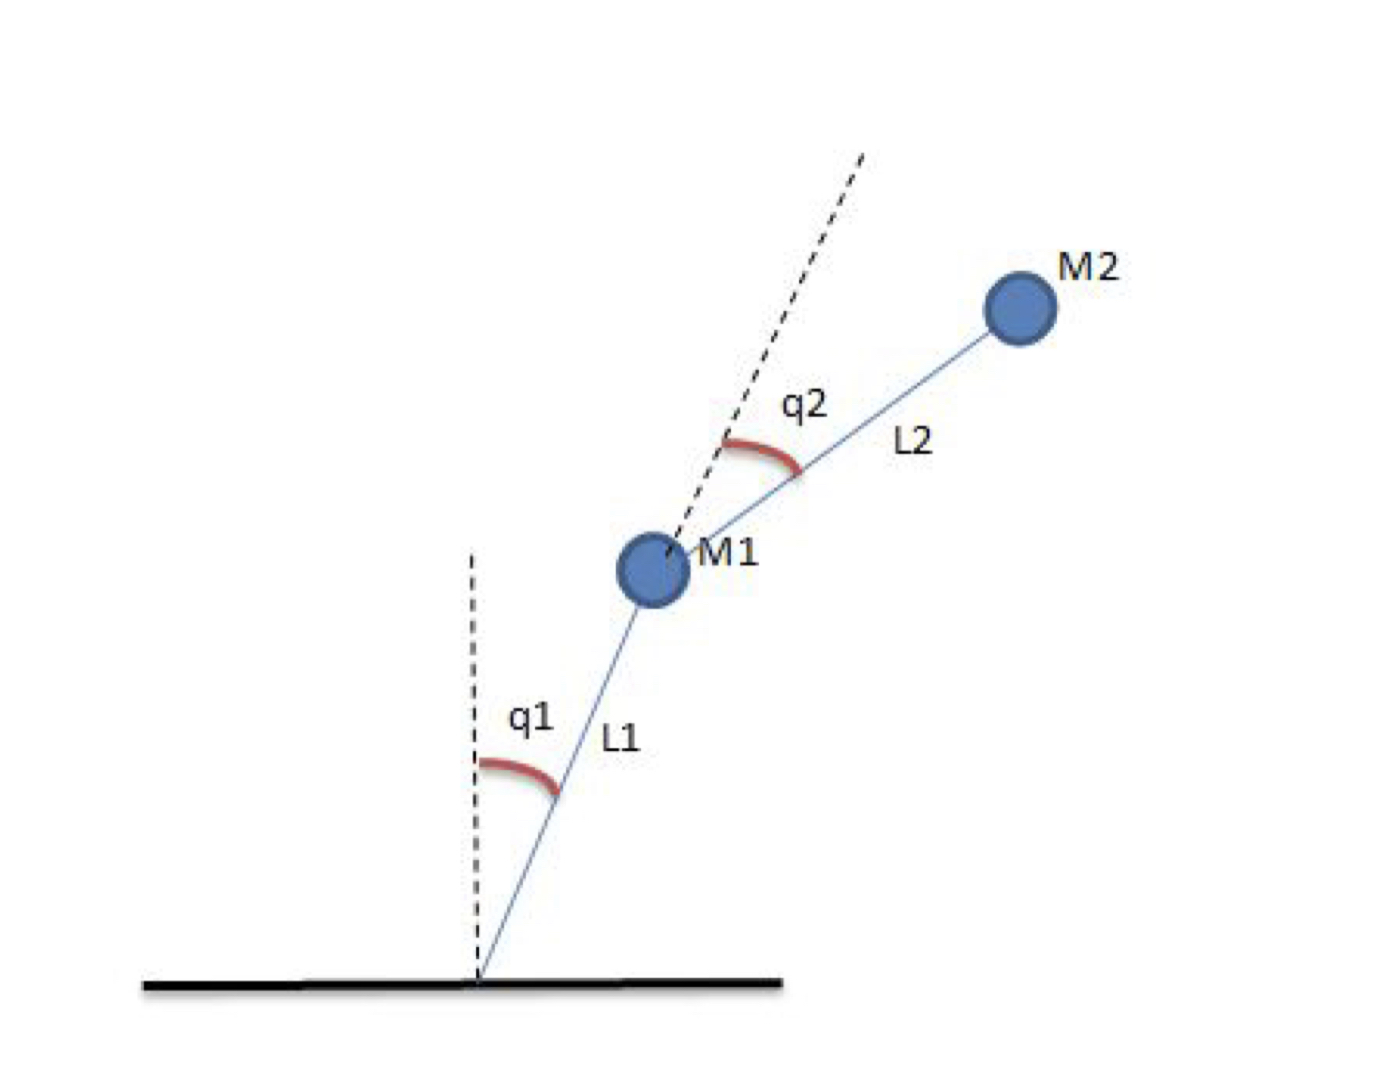
\includegraphics[scale=0.15]{images/dipm.jpeg}\hfill
    \caption{Double Inverse Pendulum Model}\hfill
    \label{dipm}
\end{figure}

Position:
\begin{equation}
\begin{split}
    x_1 &= -l_1\sin{q_1} \\
    y_1 &= l_1\cos{q_1}
\end{split}
\end{equation}

\begin{equation}
\begin{split}
    x_2 &= -l_1\sin{q_1} - l_2\sin{(q_1+q_2)} \\
    y_2 &= l_1\cos{q_1} + l_2\cos{(q_1+q_2)}
\end{split}
\end{equation}

Velocity:
\begin{equation}
\begin{split}
    \Dot{x_1} &= -l_1\cos(q_1)\Dot{q_1} \\
    \Dot{y_1} &= -l_1\sin(q_1)\Dot{q_1}
\end{split}
\end{equation}

\begin{equation}
\begin{split}
    \Dot{x_2} &= -l_1\cos(q_1)\Dot{q_1} - -l_1\cos(q_1+q_2)\Dot{(q_1+q_2)} \\
    \Dot{y_2} &= -l_1\sin(q_1)\Dot{q_1} - -l_1\sin(q_1+q_2)\Dot{(q_1+q_2)}
\end{split}
\end{equation}

Acceleration:
\begin{equation}
\begin{split}
    \Ddot{x_1} &= l_1 \sin{(q_1)}\Dot{q_1}^2 - l_1 \cos{(q_1)}\Ddot{q_1} \\
    \Ddot{y_1} &= -l_1 \cos{(q_1)}\Dot{q_1}^2 - l_1 \sin{(q_1)}\Ddot{q_1}
\end{split}
\end{equation}

\begin{equation}
\begin{split}
    \Ddot{x_2} &= -l_1\cos{(q_1)}\Ddot{q_1} + l_1\sin{(q_1)}\Dot{q_1}^2 - l_2\cos{(q_1+q_2)}(\Ddot{q_1} + \Ddot{q_2}) + l_2\sin(q_1+q_2)(\Dot{q_1} + \Dot{q_2})^2 \\
    \Ddot{y_2} &= -l_1\sin{(q_1)}\Ddot{q_1} + l_1\sin{(q_1)}\Dot{q_1}^2 - l_2\sin{(q_1+q_2)}(\Ddot{q_1} + \Ddot{q_2}) + l_2\cos(q_1+q_2)(\Dot{q_1} + \Dot{q_2})^2
\end{split}
\end{equation}

Forces and Torques:
\begin{equation}
\begin{split}
    m_1\Ddot{x_1} &= F_{x1} + F_{x_2} \\
    m_1\Ddot{y_1} &= F_{y1} + F_{y_2} - m_1g
\end{split}
\end{equation}

\begin{equation}
\begin{split}
    m_2\Ddot{x_2} &= F_{x2} \\
    m_2\Ddot{y_2} &= F_{y2} - m_2g
\end{split}
\end{equation}

where $F_{x1}$,$F_{x2}$,$F_{x3}$ and $F_{y1}$,$F_{y2}$,$F_{y3}$ represent the reaction forces on the link from the fixed point.

\begin{equation}
\begin{split}
    \tau_1 &= m_1l_1^2\Ddot{q_1} + m_1gl_1\sin{q_1} \\
    \tau_2 &= m_2l_2^2 (\Ddot{q_1} + \Ddot{q_2}) + m_2gl_2\sin(q_1+q_2)
\end{split}
\end{equation}

\subsection{Cart Table Model}
\subsection{Spherical Inverse Pendulum Approach}

\section{Approaches in Posture Control and Motion Retargetting}
\subsection{Mansard's work}
\subsection{D. Gucci's work}
\subsection{Kumar Munirathinam's work}

